\ifarxiv
\begin{figure*}[t]
	\centering
	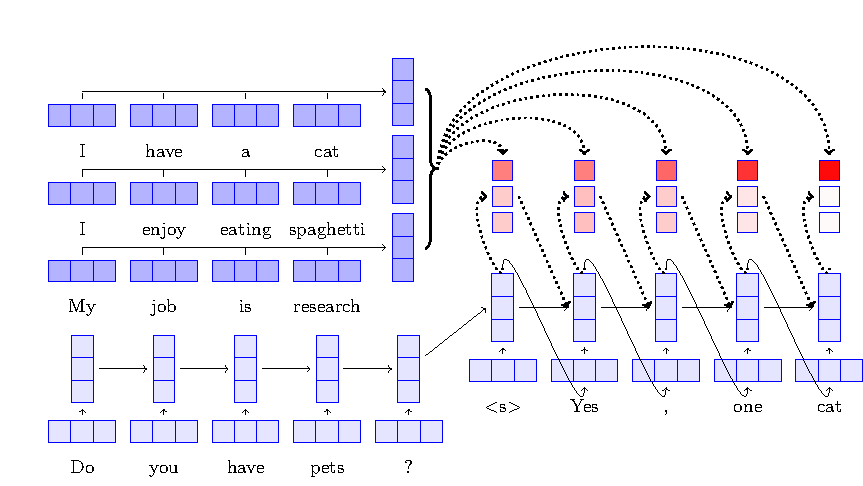
\includegraphics[width=\textwidth]{diagram.pdf}
    \caption{\label{fig:PMN-gen}A diagram of the Profile Memory Network for generation. We also implemented a ranking version which has the same architecture except it ranks candidate sentences from the training set instead of generating, representing them using bag-of-word embeddings.}
\end{figure*}
\fi

\section{Models}

We consider two classes of model for next utterance prediction: ranking models and generative models.
Ranking models produce a next utterance by considering any utterance in the training set as a possible candidate reply. Generative models 
 generate novel sentences by conditioning on the dialogue history (and possibly, the persona), and then generating the response word-by-word. % see e.g. Fig \ref{fig:PMN-gen}. 
Note one can still evaluate the latter as ranking models by computing the probability of generating a given candidate, and ranking candidates by those scores.

%Let $x$ be an input sequence (i.e., the previous dialogue utterances), $M^1$ be the set of profile entries of the speaker (i.e., the model's own profile) and $M^2$ be the profile of the listener (i.e., the interlocutor's profile). In our experiments, we compare four settings: not having access to any profile information, having access only to $M^1$, having access only to $M^2$, or having access to both $M^1 \cup M^2$. In what follows, we use $M \in \{\emptyset,M^1,M^2,M^1\cup M^2\}$ to cover all four possibilities.
%
%\subsection{Ranking Models}

%The following set of models produce a next utterance by considering any utterance in the training set as a possible candidate reply. 
%They are typically strong baselines, or, if the candidate set is big enough can be hard to beat as the sentences, being written by humans, already have fluency and internal semantic coherence. 
% On the other hand, they cannot generate novel sentences.



\ifarxiv
\subsubsection{IR Baseline}
To select candidate responses a standard baseline is nearest neighbor information retrieval (IR) (Isbell et al., 2000; Jafarpour et al., 2010; Ritter et al., 2011; Sordoni et al., 2015). 
While there are many variants, we adopt the simplest one: find the most similar message in the (training) dataset and output the response from that exchange. Similarity is measured by the tf-idf weighted cosine similarity between the bags of words. To incorporate the profile we simply concatenate it to the query vector bag of words. 


\subsubsection{Starspace}

Starspace is a recent model that performs also performs information retrieval but by learning sentence embeddings that measure similarity between the dialog and the next utterance by optimizing the word embeddings directly for that task using the training set \citep{wu2017starspace}\footnote{Available at \url{https://github.com/facebookresearch/StarSpace}}. Similar supervised embeddings have been used with good results in other dialogue tasks previously \citep{dodge2015evaluating}. 
Specifically, it optimizes:
\[
\label{math:loss}
\sum_{\substack{(q,c) \in E^+\\ b^{-} \in E^{-}}} L(sim(q, c), sim(q, c^{-}_1), \dots, sim(q, c^{-}_k))
\]
where the loss function $L$ compares a positive pair of query and candidate $(q,c)$ with the negative pairs $(q, c^{-}_i)$, $i=1,\dots, k$ using the margin ranking loss $\max(0,\mu - sim(q,c)$, where $\mu$ is the margin parameter. The similarity function $sim(\cdot, \cdot)$ is the cosine similarity of the sum of word embeddings of the query $q$ and candidate $c'$. Denoting the dictionary of ${\cal D}$ word embeddings as $W$ which is a ${\cal D} \times d$ matrix, where $W_i$ indexes the $i^{th}$ word (row), yielding its $d$-dimensional embedding, it embeds inputs $q$ and $c'$. 
  with $\sum_{i \in s} W_i$. While this model supports different word embeddings for the left and right hand side of the similarity function, we found sharing the weights gave the best performance.
  
Similar to the IR baseline, to incorporate the profile we simply concatenate it to the query vector bag of words. 
\else
\subsection{Baseline ranking models}
We first consider two baseline models, 
an IR baseline \cite{sordoni2015neural} and a supervised embedding model, Starspace \cite{wu2017starspace}\footnote{\url{github.com/facebookresearch/StarSpace}}. While there are many IR variants, we adopt the simplest one: find the most similar message in the (training) dataset and output the response from that exchange. Similarity is measured by the tf-idf weighted cosine similarity between the bags of words. 
Starspace is a recent model that also performs information retrieval but by learning %sentence embeddings (computed as the sum of  bag-of-word embeddings) that measure
the similarity
between the dialog and the next utterance by optimizing the embeddings directly for that task using the margin ranking loss and $k$-negative sampling. The similarity function $sim(q, c')$ is the cosine similarity of the sum of word embeddings of the query $q$ and candidate $c'$. Denoting the dictionary of ${\cal D}$ word embeddings as $W$ which is a ${\cal D} \times d$ matrix, where $W_i$ indexes the $i^{th}$ word (row), yielding its $d$-dimensional embedding, it embeds the sequences $q$ and $c'$.
%  with $\sum_{i \in s} W_i$.
%using the training set 
%\citep{wu2017starspace}\footnote{\tiny\url{https://github.com/facebookresearch/StarSpace}}. Similar supervised embeddings have been used with good results in other dialogue tasks previously \citep{dodge2015evaluating}. 
%%
%Specifically, it optimizes:
%\[
%\label{math:loss}
%\sum_{\substack{(q,c) \in E^+\\ b^{-} \in E^{-}}} L(sim(q, c), %sim(q, c^{-}_1), \dots, sim(q, c^{-}_k))
%\]
%where the loss function $L$ compares a positive pair of query and candidate $(q,c)$ with the negative pairs $(q, c^{-}_i)$, $i=1,\dots, k$ using the margin ranking loss $\max(0,\mu - sim(q,c)$, where $\mu$ is the margin parameter. The similarity function $sim(\cdot, \cdot)$ is the cosine similarity of the sum of word embeddings of the query $q$ and candidate $c'$. Denoting the dictionary of ${\cal D}$ word embeddings as $W$ which is a ${\cal D} \times d$ matrix, where $W_i$ indexes the $i^{th}$ word (row), yielding its $d$-dimensional embedding, it embeds a sequence $s$ 
%  with $\sum_{i \in s} W_i$.
%%

In both methods, IR and StarSpace, to incorporate the profile we simply concatenate it to the query vector bag of words. 
\fi

\subsection{Ranking Profile Memory Network}

Both the previous models use the profile information by combining it 
with the dialogue history, which means those models cannot differentiate between the two when deciding on the next utterance. In this model we instead use a memory network with the dialogue history as input, which then performs attention over the profile to find relevant lines from the profile to combine with the input, and then finally predicts the next utterance. We use the same representation and loss as in the Starspace model, so without the profile, the two models are identical.
When the profile is available attention is performed by computing the similarity of the input $q$ with the profile sentences $p_i$, computing the softmax, and taking the weighted sum:
\[
   q^+ = q + \sum s_i p_i,  ~~~~~~~~ s_i = {\mbox{Softmax}}(sim(q, p_i))
\]
where ${\mbox{Softmax}}(z_i) = e^{z_i}/\sum_j e^{z_j}$.
One can then rank the candidates $c'$ using $sim(q^+,c')$.
One can also perform multiple ``hops'' of attention over the profile rather than one, as shown here, although that did not bring significant gains in our parameter sweeps. 
%Similarly, we found a  model that shared word embedding lookup table weights across dialog history, profiles and candidates performed best compared to models with more parameters.


\subsection{Key-Value Profile Memory Network}\label{sec:kvmem}

The key-value (KV) memory network \cite{miller2016key} was proposed as an improvement to the memory network by performing attention over keys and outputting the values (instead of the same keys as in the original), which can outperform memory networks dependent on the task and definition of the key-value pairs. Here, we apply this model to dialogue, and consider the keys as dialog histories (from the training set), and the values as the next dialogue utterances, i.e., the replies from the speaking partner. 
This allows the model to have a memory of past dialogues that it can directly use to help influence its prediction for the current conversation. 
The model we choose is identical to the profile memory network just described in the first hop over profiles, while in the second hop, $q^+$ is used to attend over the keys and output a weighted sum of values as before, producing 
$q^{++}$. This is then used to rank the candidates $c'$  using $sim(q^{++},c')$ as before.  As the set of (key-value) pairs is large this would make training very slow. In our experiments we simply trained the profile memory network and used the same weights from that model and applied this architecture at test time instead. Training the model directly would presumably give better results, however this heuristic already proved beneficial compared to the original network. 

%\subsection{Generative Models}
%
%Our next set of models do generate novel sentences by conditioning on the dialogue history and possibly the persona, and then generating the response word-by-word. % see e.g. Fig \ref{fig:PMN-gen}. 
%One can still evalutate these models as ranking models by computing the probability of generating a given candidate, and ranking candidates by those scores.\footnote{In practice, better results for ranking are obtained by normalizing by the sentence length, following
% \citep{dodge2015evaluating}.}

\subsection{Seq2Seq}

The input sequence $x$ is encoded by applying $h^e_t = LSTM_{enc}(x_t \mid h^e_{t-1})$. We use GloVe \citep{pennington2014glove} for our word embeddings. The final hidden state, $h^e_t$, is fed into the decoder $LSTM_{dec}$ as the initial state $h^d_0$. For each time step $t$, the decoder then produces the probability of a word $j$ occurring in that place via the softmax, i.e.,
\begin{equation*}
p(y_{t,j} = 1 \mid y_{t-1}, \ldots, y_1) = \frac{\exp (w_j h^d_t)}{\sum^K_{j'=1} \exp (w_{j'} h^d_t)}.
\end{equation*}
The model is trained via negative log likelihood. The basic model can be extended to include persona information, in which case we simply prepend it to the input sequence $x$, i.e., $x =  \forall p \in P \mid\mid x$, where $\mid\mid$ denotes concatenation.
For the OpenSubtitles and Twitter datasets trained in Section \ref{sec:human-eval} we found training a language model (LM), essentially just the decoder part of this model, worked better and we report that instead.


\subsection{Generative Profile Memory Network}

Finally, we introduce a generative model that encodes each of the profile entries as individual memory representations in a memory network. As before, the dialogue history is encoded via $LSTM_{enc}$, the final state of which is used as the initial hidden state of the decoder. Each entry $p_i = \langle p_{i,1}, \ldots, p_{i,n} \rangle \in P$ is then encoded via $f(p_i) = \sum_j^{|p_i|} \alpha_i p_{i,j}$. That is, we weight words by their inverse term frequency: $\alpha_i = 1 / (1 + log(1 + \text{tf}))$ where $\text{tf}$ is computed from the GloVe index via Zipf's law\footnote{$\text{tf} = 1e6 * 1/(idx^{1.07})$}. Let $F$ be the set of encoded memories. The decoder now attends over the encoded profile entries, i.e., we compute the mask $a_t$, context $c_t$ and next input $\hat{x}_t$ as:
\begin{eqnarray*}
a_t = softmax(F W_a h^d_t), \\
c_t = a_t^\intercal F; ~~\hat{x}_t = tanh(W_c [c_{t-1}, x_t]).
\end{eqnarray*}
%\begin{equation}
%a_t = softmax(F W_a h^d_t)
%c_t = a_t^\intercal F; \hat{x}_t = tanh(W_c [c_{t-1}, x_t]).
%\end{equation}
\ifarxiv
This model is illustrated in Figure \ref{fig:PMN-gen}.
\fi
If the model has no profile information, and hence no memory, it becomes equivalent to the Seq2Seq model.
